%
%   Copyright 2013 Katarzyna Szawan <kat.szwn@gmail.com>
%       and Michał Rus <m@michalrus.com>
%
%   Licensed under the Apache License, Version 2.0 (the "License");
%   you may not use this file except in compliance with the License.
%   You may obtain a copy of the License at
%
%       http://www.apache.org/licenses/LICENSE-2.0
%
%   Unless required by applicable law or agreed to in writing, software
%   distributed under the License is distributed on an "AS IS" BASIS,
%   WITHOUT WARRANTIES OR CONDITIONS OF ANY KIND, either express or implied.
%   See the License for the specific language governing permissions and
%   limitations under the License.
%

\chapter{Project}
\label{chap:project}

%
%   Copyright 2013 Katarzyna Szawan <kat.szwn@gmail.com>
%       and Michał Rus <m@michalrus.com>
%
%   Licensed under the Apache License, Version 2.0 (the "License");
%   you may not use this file except in compliance with the License.
%   You may obtain a copy of the License at
%
%       http://www.apache.org/licenses/LICENSE-2.0
%
%   Unless required by applicable law or agreed to in writing, software
%   distributed under the License is distributed on an "AS IS" BASIS,
%   WITHOUT WARRANTIES OR CONDITIONS OF ANY KIND, either express or implied.
%   See the License for the specific language governing permissions and
%   limitations under the License.
%

\section{Requirements}
\label{sec:requirements}

Our aim is to create an application compatible with XMind which lets its users create, edit and display mind maps. It shoud write data in its own, native format, but also implement importing and exporting maps to XMind format. It should work on most modern Android devices, both smartphones and tablets. When it comes to functionalities, the main features are connected with managing mind maps. The most important feature (apart from these, which make it possible to use Android application) is online and offline collaboration. 

Mind maps should be presented in a clean, structured way. A special algorithm is needed to fulfill this task - the number and size of child nodes will vary. Nodes need to be positioned around the root node. Every node can have subnodes, which are displayed as a list, and it should be possible to hide or show node's whole subtree by clicking on a special button. Adding a new node can be implemented by placing a plus button on the bottom of parent node. The whole node's body should be clickable and thus a user could enter edition mode.

It should be possible to share the same map between more than one person. Every participant should be able to edit a map (online, but also when the connection is not available) and see others' changes as soon as it is possible. This feature will probably generate a number of problems with data synchronization. When f.ex. user A deletes a whole subtree online, and other, user B, being offline, changes something in the structure of the same subtree, the application should be able to recreate the deleted structure and save it as soon as user B's connection comes back. Also, it should mark any conflicts in the content of single, atomic node. 

As this is a \todo{\igor{"zły powód braku użytkowników; dobrym powodem może być to, że np. mamy inne funkcjonalności"}}proof-of-concept system, no user privileges will be implemented (although these would be easy to add, considering highly modular and clean organization of code). Thus, any device will be able to modify any existing map.


\section{Planned solution}
\label{sec:plan}

\todo[inline]{\igor{"\Cref{sec:plan} KONKRETNIE jako spełnione \cref{sec:requirements}"}}

Our application allows its users to edit maps collaboratively, either over the Internet in real time, or offline with later online synchronization. This system consists of two main components:

\begin{itemize}
	\item an Android application running on any number of Android powered devices,
	\item and a cluster of any number of servers running a distributed, highly parallelized Akka actor system with a REST interface.
\end{itemize}

%
%   Copyright 2013 Katarzyna Szawan <kat.szwn@gmail.com>
%       and Michał Rus <m@michalrus.com>
%
%   Licensed under the Apache License, Version 2.0 (the "License");
%   you may not use this file except in compliance with the License.
%   You may obtain a copy of the License at
%
%       http://www.apache.org/licenses/LICENSE-2.0
%
%   Unless required by applicable law or agreed to in writing, software
%   distributed under the License is distributed on an "AS IS" BASIS,
%   WITHOUT WARRANTIES OR CONDITIONS OF ANY KIND, either express or implied.
%   See the License for the specific language governing permissions and
%   limitations under the License.
%

\subsection{\todo{\igor{Merge with \cref{subsec:component-akka}}}Component: Android application}
\label{subsec:component-android}

\todo[inline]{\igor{"tutaj DUUUUUUŻY DIAGRAM KOMPONENTÓW używanych w części Androidowej --- UML albo ArchiMate"}}
\todo[inline]{\igor{"UI consists of: 1) OPISOWO: komponent, który daje listę --- opisowo"}}

\todo[inline]{\michal{Project Android: what subcomponents? (Own and from system library!)}}

\begin{itemize}
	\item System:
	\begin{itemize}
		\item \inlinecode{ListView}
		\item \inlinecode{TabHost} + \inlinecode{TabView}'s
		\item \todo{\michal{A lot can be written here!}}\inlinecode{ActionBarSherlock}
		\item \inlinecode{ScrollView} + \inlinecode{HorizontalScrollView} --- for our custom map view.
	\end{itemize}

	\item Own:
	\begin{itemize}
		\item \inlinecode{MainActivity} --- tabs, has fragments switchable by these tabs.
		\item \inlinecode{MapListFragment} --- alist of maps.
		\item \inlinecode{MapViewFragment}
	\end{itemize}
\end{itemize}
%
%   Copyright 2013 Katarzyna Szawan <kat.szwn@gmail.com>
%       and Michał Rus <m@michalrus.com>
%
%   Licensed under the Apache License, Version 2.0 (the "License");
%   you may not use this file except in compliance with the License.
%   You may obtain a copy of the License at
%
%       http://www.apache.org/licenses/LICENSE-2.0
%
%   Unless required by applicable law or agreed to in writing, software
%   distributed under the License is distributed on an "AS IS" BASIS,
%   WITHOUT WARRANTIES OR CONDITIONS OF ANY KIND, either express or implied.
%   See the License for the specific language governing permissions and
%   limitations under the License.
%

\subsection{Component: Akka.io application}
\label{subsec:component-akka}

Akka is used as a backend for the mobile application. It enables all mobile devices with the application installed to share maps and collaborate on them in real-time. Several REST web services are implemented using Spray.io (a REST interface to Akka) for communication between Android devices and actor system on the server-side.

Each REST-connected mobile device gets its own actor. Instant bidirectional communication between devices is achieved by means of `long-polling': mobile app initiates a connection with a REST service which does not respond until its actor receives a message from another actor. See \cref{subsec:android-akka-comm} for details about Android--Akka communication protocol.

Our Akka application consists of:

\begin{description}
	\item[Actor system]{provided by Akka framework; an environment in which all actors (of custom and system origin) live.}
	\item[Main supervisor actor]{provided by Akka; tightly integrated with the actor system. There is always one such actor for each system.}
	\item[Squeryl]{being an object-relational mapper and domain specific language for Scala and SQL databases (including PostgreSQL). Squeryl puts great emphasis on minimum verbosity and maximum type safety, as well as Don't-Repeat-Yourself principle. Created statements are validated by Scala compiler (this includes types of field). Statements that pass compilation won't fail at runtime. \cite{Squeryl:Intro}}
	\item[Database interfacing actor(s)]{that provide a persistence interface for per-user actors. Currently implemented using Squeryl.}
	\item[Spray.io based REST actors]{that manage connection between Android applications and per-user actors. These actors must encapsulate bidirectional message passing on a request-response style HTTP protocol. This is somewhat of a challenge, as described in \cref{subsec:problem-longpolling}.}
	\item[Per-user actors]{that represent a particular user/connection/device to the rest of the actor system each. By separation of these and REST actors, its is possible to easily add some other front-ends to the system. Now, the only front-end is the Android application.}
	\item[Managing actor for per-user actors]{which keeps track of all per-user actors and routes messages between them. If adding user privileges were planned, there would be no such actor (as it would be highly inefficient to check all the time which user should get which event). Instead, we would use so called `data streams' that particular per-user actors would subscribe to. Any message sent to the stream would then get automatically transmitted to all subscribed actors. Therefore a stream would represent a single mind map.}
\end{description}

The main means of communication is a `message'. This is the highest form of object-oriented model. No actor methods are called directly; instead, actors send and receive messages (similarily to Erlang's lightweight processes). Messages exchanged between different server-side actors in our system include:

\begin{itemize}
	\item Messages from \emph{REST actors} to \emph{per-user actors}:
	\begin{description}
		\item[CreateMindMap]{when user creates/imports a new mind map on their device.}
		\item[UpdateNode]{when user updates a particular node on their device. This update might be a content update, parent change, deletion.}
	\end{description}

	\item Messages from \emph{per-user actors} to \emph{DB actors}:
	\begin{description}
		\item[CreateMindMap]{}
		\item[UpdateContent]{}
		\item[UpdateParent]{}
	\end{description}

	\item Messages exchanged between \emph{managing actor} and \emph{per-user actors}, and also forwarded from \emph{per-user actors} to \emph{REST actors}:
	\begin{description}
		\item[UpdatedNode]{used to notify managing actor and other per-user actors about a particular changed node.}
	\end{description}
\end{itemize}


Again, see \cref{subsec:android-akka-comm} for details about Android--Akka communication protocol.
%
%   Copyright 2013 Katarzyna Szawan <kat.szwn@gmail.com>
%       and Michał Rus <m@michalrus.com>
%
%   Licensed under the Apache License, Version 2.0 (the "License");
%   you may not use this file except in compliance with the License.
%   You may obtain a copy of the License at
%
%       http://www.apache.org/licenses/LICENSE-2.0
%
%   Unless required by applicable law or agreed to in writing, software
%   distributed under the License is distributed on an "AS IS" BASIS,
%   WITHOUT WARRANTIES OR CONDITIONS OF ANY KIND, either express or implied.
%   See the License for the specific language governing permissions and
%   limitations under the License.
%

\subsection{Data representation}
\label{subsec:data-repr}

Mind maps edited in our software will be kept in a SQL database (\cref{fig:erd}) which consists of two tables.

\begin{enumerate}
	\item The first represents a mind map with a UUID.
	\item The second is a single `mind node' which has the following fields: \begin{itemize}
		\item UUID,
		\item its mind map's UUID,
		\item some textual content,
		\item parent node UUID,
		\item timestamp of the last modification (provided only by server, this is \emph{not a local time}; if Android modifies a node this is set to \inlinecode{NULL}; thus, local client time is \emph{never} used for synchronization protocol, as it could be set wrong),
		\item and a flag which says whether there was a merge conflict in the past, which has not yet been taken care of by the user.
	\end{itemize}
\end{enumerate}

As previously stated, we will concentrate our efforts on \emph{collaborative} aspects of the system: correct on-line synchronization in real-time as well as merging edits done off-line. As a consequence of this and a constrained time, some of the features available in the reference mind mapping software, XMind, remain yet to be implemented; see \cref{summary-future} for more details.

Both local database in Android devices (SQLite) and server-side database (PostgreSQL) share exactly the same scheme.

\begin{figure}[h]
	\centering
	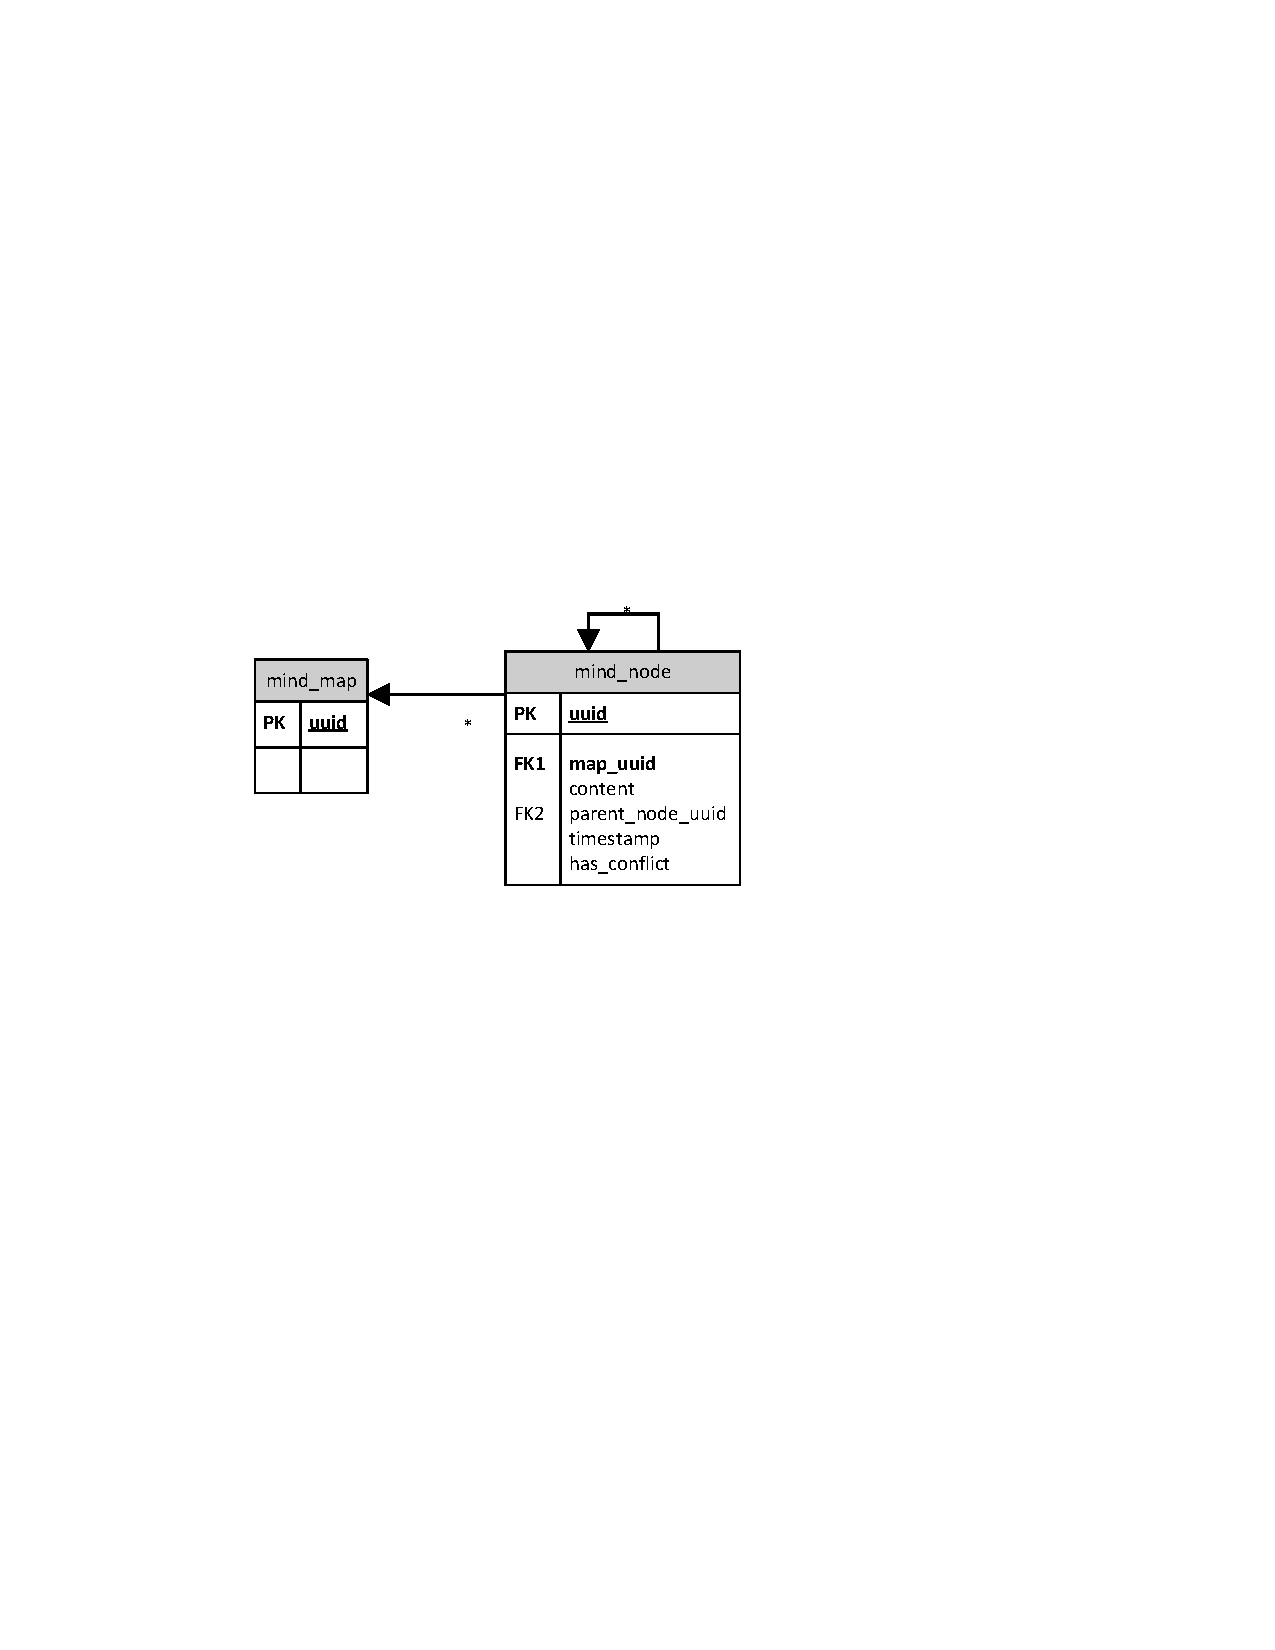
\includegraphics{graphics-erd}
	\caption{Entity relationship diagram of the database.}
	\label{fig:erd}
\end{figure}

%
%   Copyright 2013 Katarzyna Szawan <kat.szwn@gmail.com>
%       and Michał Rus <m@michalrus.com>
%
%   Licensed under the Apache License, Version 2.0 (the "License");
%   you may not use this file except in compliance with the License.
%   You may obtain a copy of the License at
%
%       http://www.apache.org/licenses/LICENSE-2.0
%
%   Unless required by applicable law or agreed to in writing, software
%   distributed under the License is distributed on an "AS IS" BASIS,
%   WITHOUT WARRANTIES OR CONDITIONS OF ANY KIND, either express or implied.
%   See the License for the specific language governing permissions and
%   limitations under the License.
%

\subsection{XMind import and export}
\label{subsec:xmind-exchange}

Details of an XMind file format can be found in \cref{sec:xmind}. XML is a way of storing data as a labeled tree created of nested tags with various attributes. Most of the attributes in  XMind tags will not be necessary, and some of them are not even used in XMind. Specifically, we want to omit data that is used to determine a style assigned to the sheet. The first step to importing an {\em XMind} file is to open it as a ZIP archive. The inlinecode{content.xml} is wrapped in an \inlinecode{InputStream}, and converted to Scala's XML object. Then, the actual parsing may be started.

Having XML support on the language level, Scala offers a very concise syntax for dealing with it~\cite{Odersky:2008:Programming}. It allows a convenient navigation through the data using \inlinecode{\textbackslash} and \inlinecode{\textbackslash\textbackslash} operators, meaning, respectively, `search in direct children' and `search in all subtags.' A content of a tag can be then obtained by using the \inlinecode{.text} method.

The \inlinecode{content.xml} file may consist of a lot of sheets (represented by \inlinecode{<sheet/>} tag with \inlinecode{id} attribute), so parsing should be done within a functional \emph{map} operation, resulting in the same number of mind maps as the number of sheets. For each sheet found, a new \inlinecode{MindMap} object is created. Then a content of the root node is set by finding sheet's first child (sheet's children are represented as \inlinecode{<topic/>}'s) and reading the content of its child, a \inlinecode{<title/>}. A single topic represents a node, which is then saved as a \inlinecode{MindNode} object. Root's children nodes are then imported recursively, using exactly the same method.

When exporting, these actions have to be reversed. First, the \inlinecode{content.xml} file is synthesized according to the rules governing the XMind format. Next, it is zipped to a file with an \inlinecode{.xmind} extension and placed on user's SD card. It's worth noting that only one file in this ZIP archive---\inlinecode{content.xml}---is absolutely sufficient to make the map readable to original XMind application.

%
%   Copyright 2013 Katarzyna Szawan <kat.szwn@gmail.com>
%       and Michał Rus <m@michalrus.com>
%
%   Licensed under the Apache License, Version 2.0 (the "License");
%   you may not use this file except in compliance with the License.
%   You may obtain a copy of the License at
%
%       http://www.apache.org/licenses/LICENSE-2.0
%
%   Unless required by applicable law or agreed to in writing, software
%   distributed under the License is distributed on an "AS IS" BASIS,
%   WITHOUT WARRANTIES OR CONDITIONS OF ANY KIND, either express or implied.
%   See the License for the specific language governing permissions and
%   limitations under the License.
%
\subsection{REST}
\label{subsec:restful}
 Communication between Android devices and actor system on the server-side requires a REST web service with two paths using the DSL of Spray.io. It enables communication over HTTP between Akka and client applications using JSON format message. We will be using GET and POST HTTP methods in order to request and send updates. Default JSON format provided by Spray.io is not sufficient for sending our application's data, so we will need custom JSON.  
 

\subsection{Communication}
\label{subsec:android-akka-comm}

Real-time collaboration (along with \emph{offline} synchronization) is by any means the most challenging part of designing and later implementing the system.

It needs mentioning that our solution is not really based on any of the existing ones. It is being created completely and from scratch by us. Such a highly parallelized system is hard to formally reason about and is yet to be proved (However, counting on a \emph{very strict} Scala compiler along with proper types and abstractions, later turned out to be a sufficient `kind-of-proof,' as the implementation works correctly. This is often a case with languages which favor immutability and functional programming: if it compiles, then it is correct). The solution will be verified in testing the application. 

As it turns out, we are able to make it work using just two main messages (and resolving two exceptional cases). However, the fact that a single node remembers only its parent will cause a number of problems with merge conflicts dealing with node deletions (solved by subtree recreation algorithm in \cref{subsec:subtree-recreation}). Communication with an Android device from the \emph{moment it gets online} is described below.

\begin{enumerate}
	\item Android looks for the newest timestamp in \inlinecode{mind\_node} table. This is the last time we had contact with Akka.

	\item Android sends a message to Akka. The message contains:
	\begin{itemize}
		\item request for all changes that happened after that \emph{newest timestamp},
		\item all local changes, that is a list of all nodes that have their timestamp set to \inlinecode{NULL}. This list of modified nodes needs to be sorted so that \emph{parents} come before \emph{children} for any two nodes in the list. \Cref{akka-unknown-parent} of exceptional cases below explains why.
	\end{itemize}

	\item Akka receives the message and:
	\begin{itemize}
		\item creates mind map(s) of UUID contained in node's map UUID field (if they don't already exists),
		\item checks if the DB will be in consistent state after introducing Android's changes. DB is said to be inconsistent when there are references in node's parent field to other nodes that are not present in DB (dangling references),
		\item any deletions are rejected if there is a previously synchronized change in to-be-deleted subtree (in such case this to-be-deleted subtree is sent again to the deleter in message in \cref{akka-update-message}),
		\item changes are merged if consistency will be retained afterwards, node's timestamps are set to current server time,
		\item if, however, consistency cannot be retained, Akka behaves in accordance to \cref{akka-unknown-parent} of exceptional cases below.
		\item There's also a possibility of a conflict, see \cref{akka-conflict} of exceptional cases below.
	\end{itemize}

	\item \label{akka-update-message} After any change to server-side DB, Akka notifies all connected Androids, including the one that initiated the change. The notification message contains all changed nodes sorted in aforementioned parent-first order.

	\item Android, after receiving this update message, updates its local DB.
\end{enumerate}

These aforementioned two exceptional cases are described below.

\begin{enumerate}
	\item \label{akka-conflict} It might happen that another Android, A, updated a node, when currently synchonizing Android, B, was offline (and B, too, changed the node while offline). This causes a `merge conflict'. All merge conflicts are resolved automatically and strategies vary depeneding on which field causes the conflict:
	\begin{itemize}
		\item if there is a conflict in node's \emph{content}, then both conflicting contents are concatenated with a new line, \inlinecode{\textbackslash{}m} and the node's \inlinecode{has\_conflict} field is set to \inlinecode{true} (this results in marking the field somehow in the UI, possibly with red),
		\item if, however, the conflicting field is node's \inlinecode{parent}, then we \emph{repin} the node accordnig to our last disposition. Changing node's parent does not destroy data and it is easy to reverse for contributors.
	\end{itemize}

	\item \label{akka-unknown-parent} It is possible that Akka will get an update request with a node which parent is \emph{not} in the DB. This might happen for two reasons:
	\begin{itemize}
		\item malicious request,
		\item or, more probably, the request is trying to update a subtree that was previously deleted (and this deletion was not synchronized at the moment of `physical' update).
	\end{itemize}

	List of updated nodes send in the request is sorted in parent-first order. This allows for a performance boost at receiving site. Akka needs only to look at modified node list's head to check whether it knows about parents of updated nodes.

	In the second case, subtree recreation algorithm has to be used (\cref{subsec:subtree-recreation}).
\end{enumerate}


%
%   Copyright 2013 Katarzyna Szawan <kat.szwn@gmail.com>
%       and Michał Rus <m@michalrus.com>
%
%   Licensed under the Apache License, Version 2.0 (the "License");
%   you may not use this file except in compliance with the License.
%   You may obtain a copy of the License at
%
%       http://www.apache.org/licenses/LICENSE-2.0
%
%   Unless required by applicable law or agreed to in writing, software
%   distributed under the License is distributed on an "AS IS" BASIS,
%   WITHOUT WARRANTIES OR CONDITIONS OF ANY KIND, either express or implied.
%   See the License for the specific language governing permissions and
%   limitations under the License.
%

\subsection{Subtree recreation algorithm}
\label{subsec:subtree-recreation}

This algorithm has to be used on the server-side, in case of a scenario described below.

\begin{enumerate}
	\item At least two users (Alice and Bob) share a map.
	\item The map gets synchronized on their devices in common state A.
	\item Alice goes offline.
	\item Bob, still online, deletes subtree S (changes state to B).
	\item Alice, still offline edits one of of children nodes in subtree S (changes state to B').
	\item Alice goes online and tries to synchronize.
	\item Server does not know a UUID of the children node, thus cannot naïvely merge B and B'.
	\item Now, subtree S has to be somehow recreated from Alice's version.
\end{enumerate}

The following steps then need to be taken:

\begin{enumerate}
	\item Akka, after receiving an update message and finding out that it does not know \emph{some} parents, responds with a request to resend the message, but, this time, with with full `genealogy' of the unknown parents.
	\item Android resends this update message at the same time adding a list of lists of parents up to the root node.
	\item Akka then knows where the lost subtrees were attached to and sends one more request for them.
	\item Android responds with original update message along with full requested subtrees from its local storage.
	\item Akka updates its DB and notifies all connected devices about the changes.
\end{enumerate}

\todo[inline]{\igor{Any proof that the algorithms work?}}

%
%   Copyright 2013 Katarzyna Szawan <kat.szwn@gmail.com>
%       and Michał Rus <m@michalrus.com>
%
%   Licensed under the Apache License, Version 2.0 (the "License");
%   you may not use this file except in compliance with the License.
%   You may obtain a copy of the License at
%
%       http://www.apache.org/licenses/LICENSE-2.0
%
%   Unless required by applicable law or agreed to in writing, software
%   distributed under the License is distributed on an "AS IS" BASIS,
%   WITHOUT WARRANTIES OR CONDITIONS OF ANY KIND, either express or implied.
%   See the License for the specific language governing permissions and
%   limitations under the License.
%

\subsection{User interface mock-ups}
\label{subsec:ui-mockups}

\Cref{fig:mockup-maplist} below show a \emph{mock-up} (a sketch) of the main, initial screen of the Android application. The user can:

\begin{itemize}
	\item choose an existing map to edit,
	\item select and delete a map by long-pressing it,
	\item add a new map,
	\item import an existing XMind map,
	\item switch to any other opened map by means of tabs at the top.
\end{itemize}

\begin{figure}[h]
	\centering
	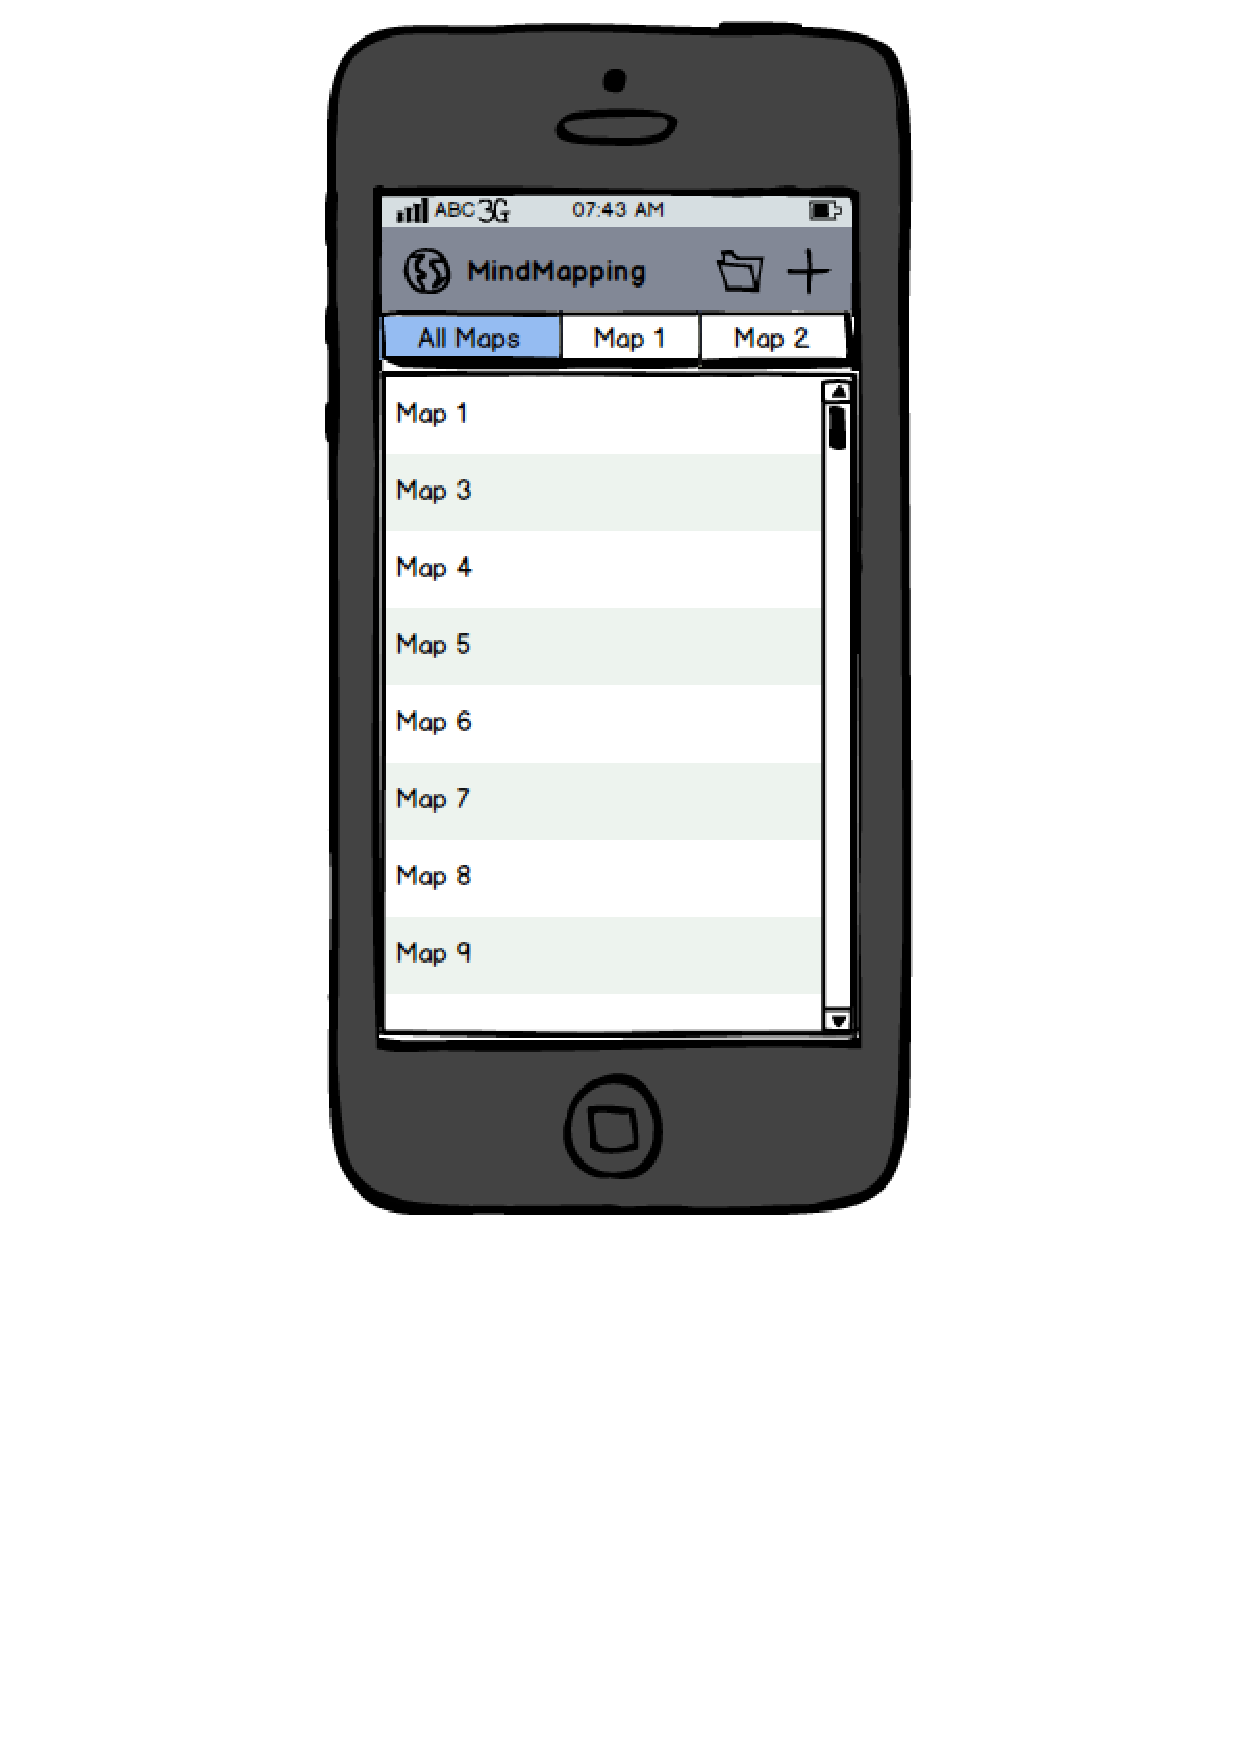
\includegraphics[width=0.5\textwidth]{graphics-mockup-list}
	\caption{Mock-up of mind map list, initial screen.}
	\label{fig:mockup-maplist}
\end{figure}

\Cref{fig:mockup-mindmap} shows a similar preview of a map view: a screen that is shown to the user when he chooses/adds/imports a map in \cref{fig:mockup-maplist}. Here, the user can:

\begin{itemize}
	\item edit content of any `mind node' by tapping on it,
	\item remove any node (and its subtree) by long-pressing it and selecting `remove',
	\item move any node (reassign its parent node) by long-pressing it and selecting `change parent', and then tapping on the new parent,
	\item add a child node to any node by tapping on `+' button next to the parent node,
	\item see (in real-time) changes introduced by other editors currently editing this map.
\end{itemize}

\begin{figure}[h]
	\centering
	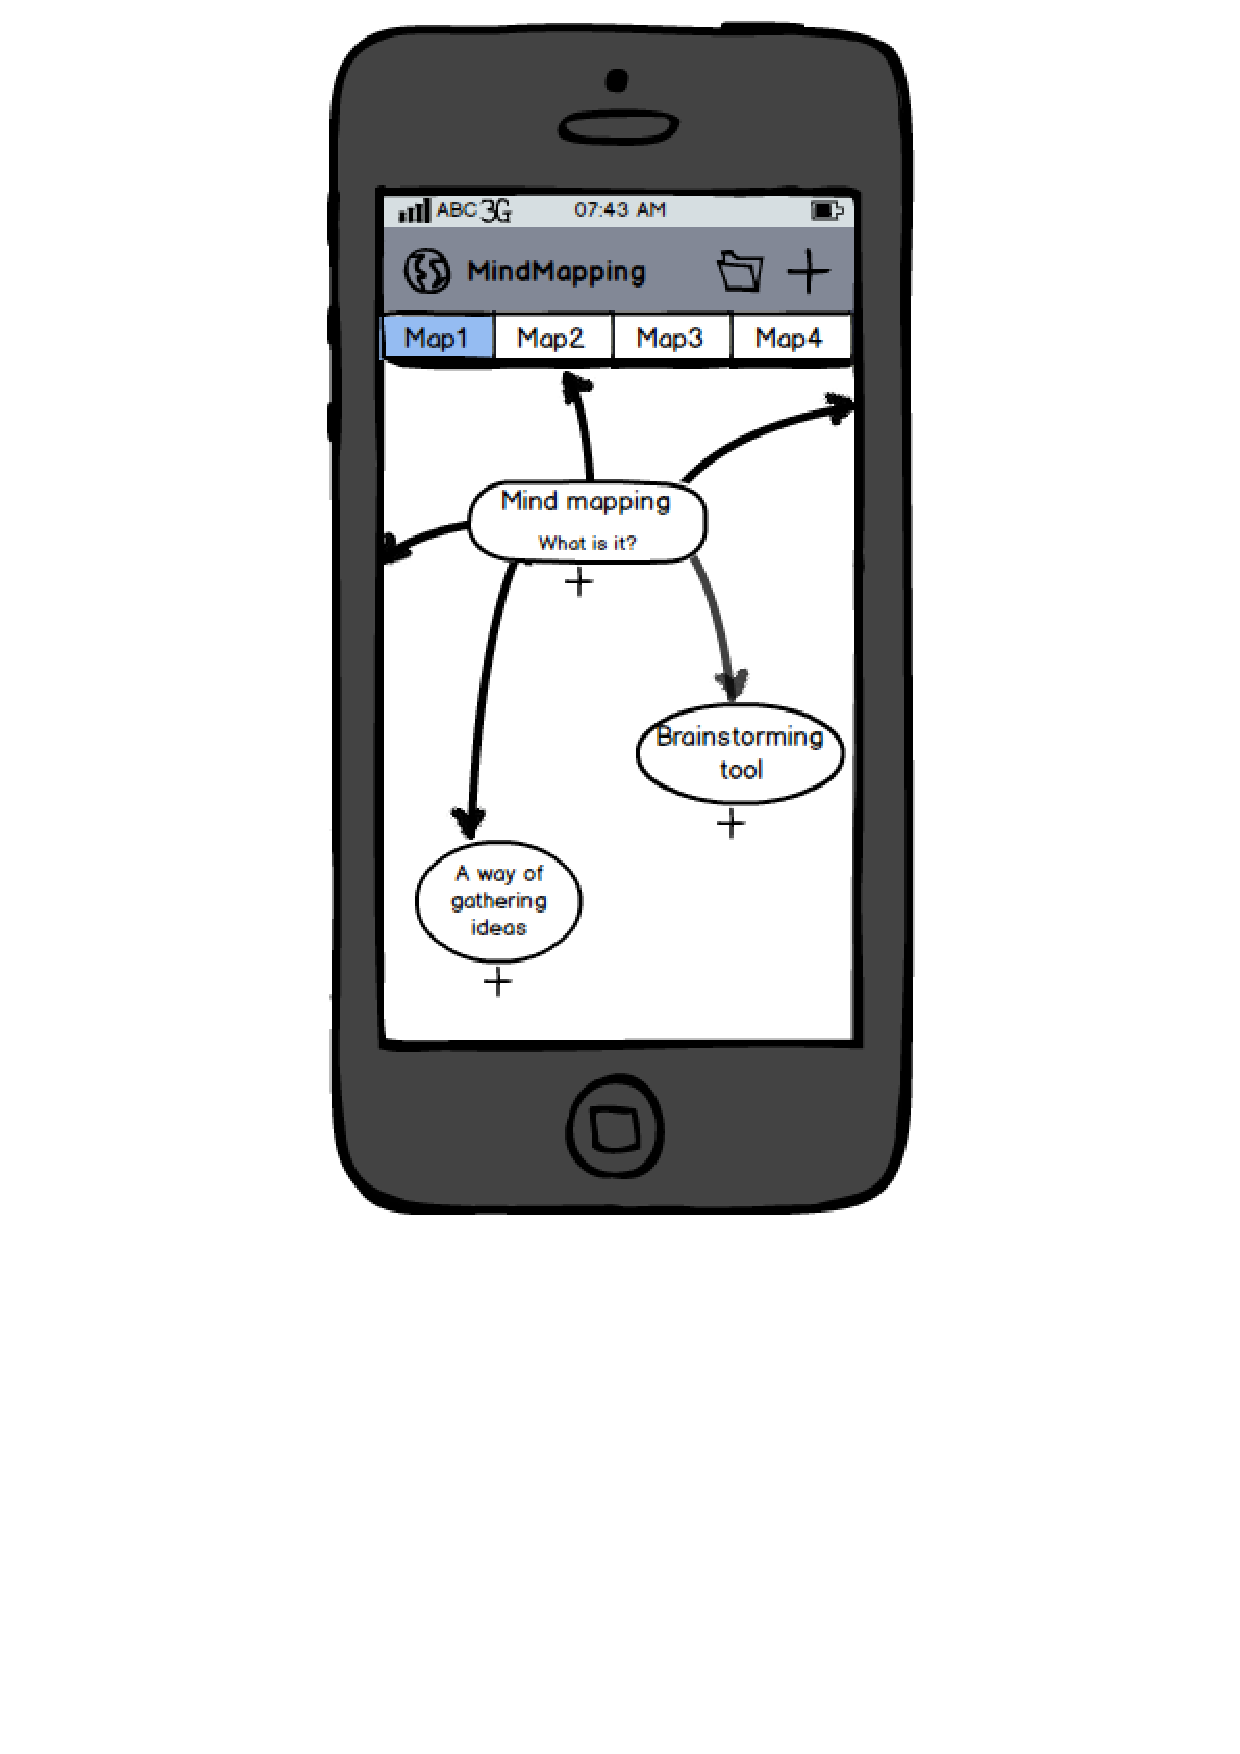
\includegraphics[width=0.5\textwidth]{graphics-mockup-map}
	\caption{Mock-up of mind map view.}
	\label{fig:mockup-mindmap}
\end{figure}

\todo[inline,caption=\michal{K., any more mock-ups needed?}
\kasia{I think it's enough. Now we need to fit the size of the images}]{}

